%!TEX program = pdflatex
% Guide d'utilisation de l'espace administrateur de CamerRideShare.
% Compilation : latexmk -pdf guide-admin.tex   (deux passes pour la table des matières et les renvois)
% Les captures sont régénérées avec capture/capture.mjs (voir README.md).
\documentclass[11pt,a4paper]{article}

\usepackage[utf8]{inputenc}
\usepackage[T1]{fontenc}
\usepackage[french]{babel}
\usepackage{helvet}
\renewcommand{\familydefault}{\sfdefault}
\usepackage[a4paper,left=2.3cm,right=2.3cm,top=2.6cm,bottom=2.4cm]{geometry}
\usepackage{xcolor}
\usepackage{graphicx}
\usepackage{float}
\usepackage{caption}
\usepackage{enumitem}
\usepackage{booktabs}
\usepackage{array}
\usepackage{tabularx}
\usepackage{fancyhdr}
\usepackage{titlesec}
\usepackage{tikz}
\usetikzlibrary{arrows.meta,positioning,shapes.geometric,calc,fit}
\usepackage[most]{tcolorbox}
\usepackage[hidelinks]{hyperref}
\usepackage{microtype}
\usepackage{etoolbox}
% Saut de page si la place restante est insuffisante (équivalent de needspace, sans extension supplémentaire)
\newcommand{\Needspace}[1]{\par\ifdim\pagegoal<\maxdimen\ifdim\dimexpr\pagegoal-\pagetotal\relax<#1\relax\newpage\fi\fi}
\AtBeginEnvironment{tabularx}{\setlength{\parskip}{0pt}}
\newcolumntype{L}[1]{>{\bfseries\raggedright\arraybackslash\textcolor{vert}\bgroup}p{#1}<{\egroup}}

% ─── Couleurs (celles de l'application) ──────────────────────────────────────
\definecolor{vert}{HTML}{148664}
\definecolor{vertclair}{HTML}{E4F3EE}
\definecolor{marque}{HTML}{E8590C}   % couleur des pastilles et des cadres sur les captures
\definecolor{marqueclair}{HTML}{FFF1E8}
\definecolor{bleu}{HTML}{1D4E89}
\definecolor{bleuclair}{HTML}{E8F0FA}
\definecolor{gris}{HTML}{5B6270}
\definecolor{grisclair}{HTML}{F3F4F6}
\definecolor{rouge}{HTML}{C62828}
\definecolor{rougeclair}{HTML}{FDECEC}

\hypersetup{pdftitle={Guide d'utilisation de l'espace administrateur -- CamerRideShare},pdfauthor={Abdoulrahim Momo Aboubakar}}

% ─── Pastille numérotée (identique à celles des captures) ────────────────────
\newcommand{\mk}[1]{\tikz[baseline=(c.base)]\node[circle,fill=marque,text=white,inner sep=0pt,minimum size=1.45ex+3pt,font=\bfseries\scriptsize\sffamily,draw=white,line width=0.4pt] (c) {#1};}

% Légende d'une capture : liste de pastilles expliquées
\newenvironment{legende}{\begin{list}{}{\setlength{\leftmargin}{2.1em}\setlength{\labelwidth}{1.8em}\setlength{\labelsep}{0.3em}\setlength{\itemsep}{2pt}\setlength{\topsep}{4pt}\setlength{\parsep}{0pt}\renewcommand{\makelabel}[1]{\hss##1}}}{\end{list}}

% Capture : \capture{fichier}{etiquette}{légende}{hauteur max en fraction de la page}
\newcommand{\capture}[4]{%
  \Needspace{\dimexpr#4\textheight+3.2cm\relax}
  \begin{figure}[H]\centering
  \fcolorbox{gris!45}{white}{\includegraphics[width=\linewidth,height=#4\textheight,keepaspectratio]{images/#1}}
  \caption{#3}\label{fig:#2}
  \end{figure}}

% Deux captures côte à côte (téléphone)
\newcommand{\captureduo}[5]{%
  \Needspace{\dimexpr#5\textheight+3.2cm\relax}
  \begin{figure}[H]\centering
  \fcolorbox{gris!45}{white}{\includegraphics[height=#5\textheight]{images/#1}}\hspace{1.2cm}%
  \fcolorbox{gris!45}{white}{\includegraphics[height=#5\textheight]{images/#2}}
  \caption{#4}\label{fig:#3}
  \end{figure}}

% ─── Encadrés ────────────────────────────────────────────────────────────────
\newtcolorbox{astuce}{enhanced,breakable,colback=vertclair,colframe=vert,boxrule=0.6pt,leftrule=3.5pt,arc=2pt,
  top=9pt,bottom=5pt,left=6pt,right=6pt,before skip=14pt,after skip=10pt,
  title={\textbf{Astuce}},coltitle=vert,colbacktitle=vertclair,fonttitle=\sffamily,attach boxed title to top left={yshift=-2.5mm,xshift=3mm},
  boxed title style={colback=white,colframe=vert,boxrule=0.5pt,arc=2pt,top=1pt,bottom=1pt}}
\newtcolorbox{attention}{enhanced,breakable,colback=rougeclair,colframe=rouge,boxrule=0.6pt,leftrule=3.5pt,arc=2pt,
  top=9pt,bottom=5pt,left=6pt,right=6pt,before skip=14pt,after skip=10pt,
  title={\textbf{Attention}},coltitle=rouge,colbacktitle=rougeclair,fonttitle=\sffamily,attach boxed title to top left={yshift=-2.5mm,xshift=3mm},
  boxed title style={colback=white,colframe=rouge,boxrule=0.5pt,arc=2pt,top=1pt,bottom=1pt}}
\newtcolorbox{retenir}{enhanced,breakable,colback=bleuclair,colframe=bleu,boxrule=0.6pt,leftrule=3.5pt,arc=2pt,
  top=9pt,bottom=5pt,left=6pt,right=6pt,before skip=14pt,after skip=10pt,
  title={\textbf{À retenir}},coltitle=bleu,colbacktitle=bleuclair,fonttitle=\sffamily,attach boxed title to top left={yshift=-2.5mm,xshift=3mm},
  boxed title style={colback=white,colframe=bleu,boxrule=0.5pt,arc=2pt,top=1pt,bottom=1pt}}

% Étapes numérotées
\setlist[enumerate,1]{label=\textbf{\textcolor{vert}{\arabic*.}},leftmargin=2em,itemsep=3pt,topsep=4pt}
\setlist[itemize,1]{leftmargin=1.6em,itemsep=2pt,topsep=4pt}
% Nom d'un bouton ou d'un menu, tel qu'il apparaît à l'écran
\newcommand{\bouton}[1]{\textbf{«\,#1\,»}}

% ─── Titres ──────────────────────────────────────────────────────────────────
\titleformat{\section}{\color{vert}\normalfont\sffamily\huge\bfseries}{\thesection}{0.6em}{}[\vspace{3pt}\color{vert}\titlerule]
\titleformat{\subsection}{\color{bleu}\normalfont\sffamily\Large\bfseries}{\thesubsection}{0.6em}{}
\titleformat{\subsubsection}{\color{gris}\normalfont\sffamily\large\bfseries}{}{0em}{}
\titlespacing*{\section}{0pt}{0pt}{14pt}
\titlespacing*{\subsection}{0pt}{16pt}{6pt}
\titlespacing*{\subsubsection}{0pt}{10pt}{3pt}
\captionsetup{font={small,sf},labelfont={bf,color=vert},labelsep=period,justification=centering,skip=6pt}

% Un titre de sous-section n'est jamais isolé en bas de page
\let\oldsubsection\subsection
\renewcommand{\subsection}{\Needspace{10.5cm}\oldsubsection}
% Chaque section (chapitre) commence sur une nouvelle page
\let\oldsection\section
\renewcommand{\section}{\clearpage\oldsection}

% ─── En-têtes ────────────────────────────────────────────────────────────────
\pagestyle{fancy}
\fancyhf{}
\renewcommand{\headrulewidth}{0.4pt}
\renewcommand{\footrulewidth}{0pt}
\fancyhead[L]{\small\color{gris}CamerRideShare -- Guide de l'administrateur}
\fancyhead[R]{\small\color{gris}\nouppercase{\leftmark}}
\fancyfoot[C]{\small\color{gris}Page \thepage}
\setlength{\headheight}{14pt}
\setlength{\parindent}{0pt}
\setlength{\parskip}{5pt plus 1pt}
\renewcommand{\arraystretch}{1.25}

\begin{document}

% ═══ PAGE DE GARDE ═══════════════════════════════════════════════════════════
\begin{titlepage}
\thispagestyle{empty}
\begin{tikzpicture}[remember picture,overlay]
  \fill[vert] (current page.north west) rectangle ([yshift=-11.2cm]current page.north east);
  \fill[marque] ([yshift=-11.2cm]current page.north west) rectangle ([yshift=-11.55cm]current page.north east);
  \node[anchor=north west,inner sep=0pt] at ([xshift=2.3cm,yshift=-2.2cm]current page.north west) {
\includegraphics[height=2.6cm]{images/logo.png}};
  \node[anchor=north west,text=white,align=left,inner sep=0pt] at ([xshift=2.3cm,yshift=-5.6cm]current page.north west)
    {{\sffamily\fontsize{34}{40}\selectfont\bfseries Guide d'utilisation}\\[6pt]{\sffamily\fontsize{22}{26}\selectfont Espace administrateur}};
  \node[anchor=north west,text=white,inner sep=0pt] at ([xshift=2.3cm,yshift=-9.4cm]current page.north west)
    {\sffamily\large CamerRideShare -- gestion de motos-taxis, de conducteurs et d'investisseurs};
\end{tikzpicture}

\vspace*{10.2cm}

{\large Ce guide s'adresse à toute personne qui administre la plateforme, \textbf{sans aucune connaissance technique requise} : chaque écran est présenté pas à pas, avec des captures annotées.}

\vspace{1.2cm}
\begin{tcolorbox}[colback=grisclair,colframe=grisclair,arc=3pt,left=10pt,right=10pt,top=8pt,bottom=8pt]
\begin{tabularx}{\linewidth}{@{}L{3.2cm}X@{}}
Auteur & Abdoulrahim Momo Aboubakar\\
Version & 1.0 -- novembre 2026\\
Application & CamerRideShare, portail administrateur\\
Données & Les captures ont été réalisées avec des données fictives de démonstration.\\
\end{tabularx}
\end{tcolorbox}
\end{titlepage}

\tableofcontents
\clearpage

% ═══ AVANT-PROPOS ════════════════════════════════════════════════════════════
\section*{Comment utiliser ce guide}
\addcontentsline{toc}{section}{Comment utiliser ce guide}
\markboth{Comment utiliser ce guide}{Comment utiliser ce guide}

Ce guide vous accompagne de votre première connexion jusqu'à la gestion quotidienne de la plateforme. Vous n'avez pas besoin de le lire d'un trait : chaque chapitre correspond à une page du logiciel, et vous pouvez aller directement à celui dont vous avez besoin (voir aussi l'\hyperref[sec:taches]{index des tâches courantes} à la fin).

\subsection*{Les repères sur les captures d'écran}

Sur chaque capture, les zones importantes sont entourées d'un \textbf{cadre orange} et numérotées avec une \textbf{pastille orange} comme celle-ci : \mk{1}. Le texte situé sous la capture explique ce que chaque numéro désigne.

\subsection*{Les encadrés}

\begin{astuce}
Un conseil pour aller plus vite ou éviter une erreur courante.
\end{astuce}
\begin{attention}
Une action importante ou difficile à annuler : lisez-la avant de cliquer.
\end{attention}
\begin{retenir}
L'essentiel d'une notion, à garder en tête.
\end{retenir}

\subsection*{Les mots employés à l'écran}

Les noms entre guillemets, par exemple \bouton{Saisir un paiement}, sont écrits exactement comme dans le logiciel : cherchez-les à l'écran. Le logiciel s'utilise avec la souris ou, sur téléphone et tablette, avec le doigt ; « cliquer » signifie aussi « toucher ».

% ═══ 1. COMPRENDRE ═══════════════════════════════════════════════════════════
\section{Comprendre CamerRideShare en cinq minutes}

\subsection{À quoi sert la plateforme ?}

CamerRideShare organise le financement et l'exploitation de motos-taxis et de taxis au Cameroun. Trois types de personnes utilisent la plateforme, chacun avec son propre espace :

\begin{center}
\begin{tabularx}{\linewidth}{@{}>{\bfseries}p{3.2cm}X@{}}
\toprule
\textcolor{vert}{Administrateur} & \textbf{Vous.} Vous gérez les véhicules, encaissez les versements des conducteurs, reversez leurs gains aux investisseurs et suivez les retards. Vous avez accès à tout.\\
\midrule
\textcolor{vert}{Conducteur} & Il conduit un véhicule et le rembourse chaque semaine. Il déclare ses versements depuis son téléphone, éventuellement avec la photo de la preuve de paiement.\\
\midrule
\textcolor{vert}{Investisseur} & Il finance une partie du prix d'achat d'un véhicule (une « part ») et reçoit ensuite sa part des versements du conducteur.\\
\bottomrule
\end{tabularx}
\end{center}

\subsection{Le circuit de l'argent}

\begin{center}
\begin{tikzpicture}[
  node distance=1.0cm and 1.6cm,
  box/.style={rounded corners=3pt,draw=vert,fill=vertclair,align=center,minimum height=1.15cm,minimum width=3.0cm,font=\small\sffamily},
  adm/.style={rounded corners=3pt,draw=marque,fill=marqueclair,align=center,minimum height=1.15cm,minimum width=3.0cm,font=\small\sffamily\bfseries},
  fleche/.style={-{Stealth[length=2.4mm]},thick,color=gris},
  lab/.style={font=\scriptsize\sffamily\itshape,color=gris,align=center}]
  \node[box] (inv) {Investisseurs};
  \node[adm,right=of inv] (adm) {Vous\\(administrateur)};
  \node[box,right=of adm] (veh) {Véhicule};
  \node[box,below=1.5cm of veh] (cond) {Conducteur};
  \node[box,below=1.5cm of inv] (rev) {Reversements};
  \draw[fleche] (inv) -- node[lab,above]{apports\\(parts)} (adm);
  \draw[fleche] (adm) -- node[lab,above]{achat} (veh);
  \draw[fleche] (veh) -- node[lab,right]{confié à} (cond);
  \draw[fleche] (cond) -- node[lab,above]{versements\\chaque semaine} (adm |- cond) -- (adm);
  \draw[fleche] (adm) -- ++(0,-2.1) -| node[lab,pos=0.25,above]{gains}(rev);
  \draw[fleche] (rev) -- node[lab,left]{reçus par} (inv);
\end{tikzpicture}
\end{center}

\begin{enumerate}
  \item Les investisseurs apportent de l'argent sous forme de \textbf{parts}. Ces parts financent l'achat du véhicule.
  \item Le véhicule est confié à un conducteur, qui verse un montant fixe \textbf{chaque semaine}.
  \item Vous encaissez ces versements, puis \textbf{reversez} aux investisseurs leur part, chaque semaine ou chaque mois selon leur choix.
\end{enumerate}

\subsection{Un exemple chiffré}

\begin{retenir}
Le conducteur rembourse \textbf{160\,\%} du prix d'achat du véhicule, par versements hebdomadaires. Chaque investisseur reçoit \textbf{160\,\% de son apport}, au prorata de sa part.
\end{retenir}

Prenons une moto achetée \textbf{550\,000~XAF} (le franc CFA, ou XAF, est la monnaie utilisée partout dans le logiciel) :

\begin{center}
\begin{tabularx}{0.92\linewidth}{@{}Xr@{}}
\toprule
\textbf{Montant à rembourser par le conducteur} (160\,\% de 550\,000) & \textbf{880\,000~XAF}\\
Versement hebdomadaire fixé par vous & 27\,500~XAF\\
Durée du contrat (880\,000 $\div$ 27\,500) & 32 semaines\\
\midrule
Part d'un investisseur qui a apporté 110\,000~XAF (20\,\% du prix) & \\
\quad ses gains à chaque versement du conducteur (20\,\% de 27\,500) & 5\,500~XAF\\
\quad ses gains au total (160\,\% de 110\,000) & 176\,000~XAF\\
\bottomrule
\end{tabularx}
\end{center}

\subsection{Les mots à connaître}

\begin{center}
\begin{tabularx}{\linewidth}{@{}L{3.4cm}X@{}}
\toprule
Part & L'apport d'un investisseur sur un véhicule (minimum 50\,000~XAF). Un investisseur peut avoir plusieurs parts, y compris sur le même véhicule. Chaque part est un contrat à part entière.\\
Montant cible & Ce que le conducteur doit rembourser au total (160\,\% du prix d'achat).\\
Versement & Ce que le conducteur paie chaque semaine.\\
Retard & Une semaine pour laquelle le conducteur n'a pas versé la somme due. Chaque retard \textbf{ajoute une semaine} à la fin de son calendrier.\\
Reversement & L'argent que vous remettez à un investisseur (sa part des versements encaissés).\\
Tournée & La période pendant laquelle un conducteur est affecté à un véhicule.\\
Créance & Ce qu'un conducteur dont le contrat a pris fin doit encore à la société.\\
Rattrapage & Somme due à un investisseur qui entre sur un véhicule déjà en service, pour les semaines passées.\\
\bottomrule
\end{tabularx}
\end{center}

% ═══ 2. SE CONNECTER ═════════════════════════════════════════════════════════
\section{Se connecter et se repérer}

\subsection{Se connecter}

L'adresse du logiciel est celle que l'on vous a communiquée (par exemple \texttt{camerrideshare.strife-cyber.org}). Vous pouvez l'ouvrir dans n'importe quel navigateur, sur ordinateur, tablette ou téléphone.

\capture{01-connexion.png}{connexion}{La page de connexion.}{0.5}
\begin{legende}
  \item[\mk{1}] \textbf{Numéro de téléphone} : c'est votre identifiant. Saisissez-le sans espace, par exemple \texttt{692100263}.
  \item[\mk{2}] \textbf{Mot de passe}. Le petit œil, à droite, permet de l'afficher le temps de vérifier votre saisie.
  \item[\mk{3}] \textbf{Se connecter} : ouvre votre espace. Le bouton reste grisé tant que les deux champs ne sont pas remplis.
  \item[\mk{4}] Rappel : l'accès se fait \textbf{sur invitation}. Il n'y a pas de création de compte libre.
\end{legende}

\begin{attention}
Après plusieurs tentatives ratées, la connexion est bloquée quelques minutes par sécurité (dix essais sur quinze minutes). Si cela arrive, patientez avant de réessayer. Ne communiquez jamais votre mot de passe : personne n'a besoin de vous le demander.
\end{attention}

\begin{astuce}
Mot de passe oublié ? Un autre administrateur peut le réinitialiser pour vous (voir \autoref{sec:acces}, « Gestion des accès »).
\end{astuce}

\subsection{L'écran en un coup d'œil}

Toutes les pages de l'espace administrateur ont la même organisation.

\capture{02-reperes.png}{reperes}{Les zones communes à toutes les pages.}{0.5}
\begin{legende}
  \item[\mk{1}] \textbf{Le menu} : neuf entrées, une par page (tableau de bord, parc, paiements, investisseurs, demandes de parts, reversements, calendrier, retards, paramètres). La page affichée est surlignée en vert.
  \item[\mk{2}] \textbf{Le bouton de réduction} du menu : il le replie pour gagner de la place, ou le rouvre.
  \item[\mk{3}] \textbf{Le fil d'Ariane} : il rappelle où vous êtes.
  \item[\mk{4}] \textbf{La cloche} des notifications (voir ci-dessous). Le chiffre indique combien de notifications sont non lues.
  \item[\mk{5}] \textbf{Le bouton lune} : bascule entre le thème clair et le thème sombre, plus reposant le soir.
  \item[\mk{6}] \textbf{Votre profil} et le bouton \bouton{Déconnexion}. Pensez à vous déconnecter si vous utilisez un ordinateur partagé.
  \item[\mk{7}] \textbf{La zone de travail} : le contenu de la page choisie.
\end{legende}

\subsection{La cloche de notifications}

La cloche vous prévient des événements qui demandent votre attention : nouvel incident, paiements en attente de validation, reversements en retard, demande de part d'un investisseur, nouveau compte créé\ldots

\capture{05-cloche.png}{cloche}{La liste des notifications.}{0.42}
\begin{legende}
  \item[\mk{1}] La cloche : cliquez dessus pour ouvrir la liste.
  \item[\mk{2}] \bouton{Tout lire} marque toutes les notifications comme lues.
  \item[\mk{3}] Une notification \textbf{non lue} est surlignée et précédée d'un point jaune.
  \item[\mk{4}] Cliquez sur une notification : elle est marquée comme lue et vous amène directement à la page concernée.
\end{legende}

La liste se met à jour toute seule toutes les trente secondes environ.

\subsection{Utiliser le logiciel sur téléphone}

Le logiciel s'adapte à l'écran du téléphone : le menu se range alors derrière un bouton.

\captureduo{31-mobile-a.png}{31-mobile-b.png}{mobile}{Sur téléphone : l'écran d'accueil (à gauche) et le menu ouvert (à droite).}{0.5}
\begin{legende}
  \item[\mk{1}] Le bouton qui \textbf{ouvre le menu}.
  \item[\mk{2}] La cloche de notifications.
  \item[\mk{3}] Le thème clair ou sombre.
  \item[\mk{4}] Le menu ouvert : touchez une entrée pour changer de page.
  \item[\mk{5}] Votre profil et la déconnexion.
  \item[\mk{6}] Touchez la zone grisée, à droite, pour fermer le menu.
\end{legende}

\subsection{Installer l'application sur l'écran d'accueil}

Vous pouvez installer CamerRideShare comme une vraie application, sans passer par un magasin d'applications. Elle s'ouvre alors en plein écran, avec son icône, comme les autres.

\subsubsection*{Sur ordinateur ou sur téléphone Android}

\capture{32-installation-bureau.png}{installbureau}{Le bouton d'installation, au-dessus de « Déconnexion ».}{0.2}
\begin{enumerate}
  \item Ouvrez le menu : si votre navigateur sait installer l'application, le bouton \mk{1} \bouton{Installer l'application} apparaît juste au-dessus de \mk{2} \bouton{Déconnexion}.
  \item Cliquez dessus et confirmez dans la fenêtre du navigateur.
\end{enumerate}

\subsubsection*{Sur iPhone ou iPad}

Apple n'affiche pas de fenêtre d'installation automatique : le bouton \bouton{Installer l'application} ouvre donc une petite explication.

\begin{figure}[H]\centering
\fcolorbox{gris!45}{white}{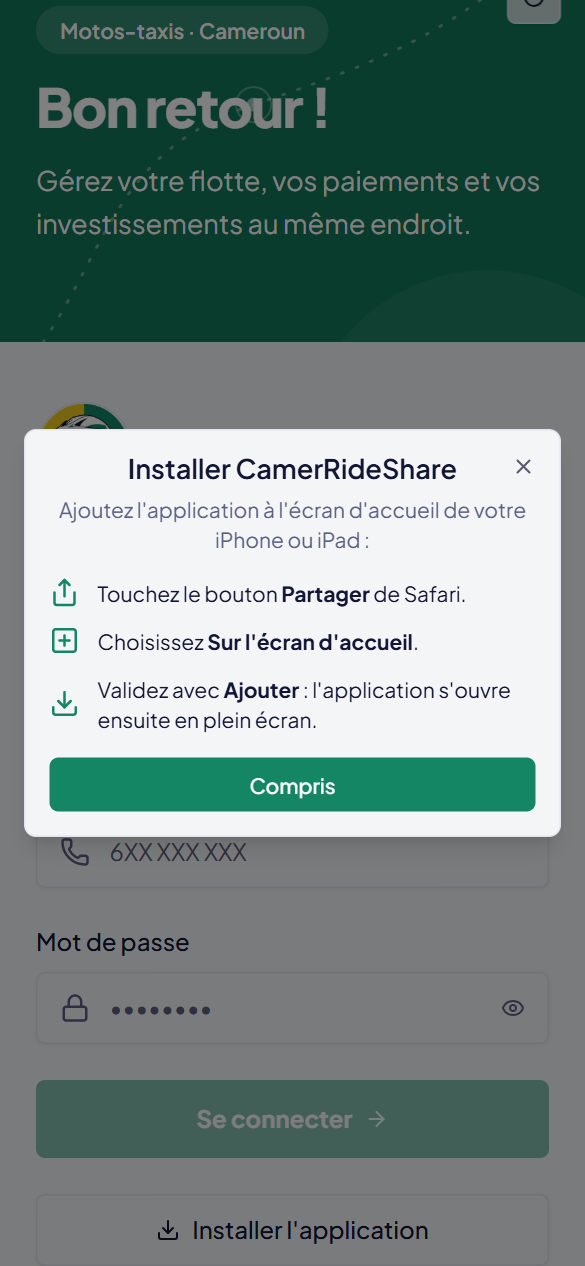
\includegraphics[height=0.42\textheight]{images/32-installation-iphone.png}}
\caption{Sur iPhone : la fenêtre d'explication.}\label{fig:iphone}
\end{figure}
\begin{enumerate}
  \item Ouvrez le logiciel dans \textbf{Safari}.
  \item Touchez le bouton \textbf{Partager} de Safari.
  \item Choisissez \bouton{Sur l'écran d'accueil}, puis \bouton{Ajouter}.
\end{enumerate}

\begin{astuce}
L'application installée \textbf{se met à jour toute seule} : à chaque nouvelle version, elle se renouvelle sans que vous ayez rien à faire. Si l'application semble figée ou affiche un écran blanc, elle essaie de se réparer d'elle-même au bout de quelques secondes ; sinon, fermez-la complètement puis rouvrez-la.
\end{astuce}

% ═══ 3. TABLEAU DE BORD ══════════════════════════════════════════════════════
\section{Le tableau de bord}

C'est la page qui s'ouvre après la connexion. Elle répond à une question : \textit{qu'est-ce qui demande mon attention aujourd'hui ?}

\capture{03-dashboard.png}{dashboard}{Le tableau de bord.}{0.62}
\begin{legende}
  \item[\mk{1}] \textbf{Les trois chiffres clés} : le \textbf{parc total} (nombre de véhicules), les \textbf{investisseurs actifs} et le \textbf{revenu mensuel}. Chaque carte indique l'évolution par rapport au mois précédent (flèche verte : en hausse ; flèche rouge : en baisse).
  \item[\mk{2}] \textbf{État du parc} : la part de véhicules en route (le grand pourcentage), avec le détail : \textit{actifs}, \textit{en panne} et \textit{volés ou perdus}.
  \item[\mk{3}] \textbf{Trésorerie hebdomadaire} : ce qui a été encaissé cette semaine par rapport à l'objectif de la semaine, avec le pourcentage « recouvré ».
  \item[\mk{4}] \textbf{Alertes critiques} : les situations à traiter en priorité (voir ci-dessous).
  \item[\mk{5}] \textbf{Actions rapides} : trois raccourcis pour les gestes les plus fréquents.
  \item[\mk{6}] \textbf{Transactions récentes} : les derniers paiements et dépenses. \bouton{Tout afficher} ouvre la page \bouton{Paiements}.
\end{legende}

\subsection{Comprendre les alertes}

Le bloc \bouton{Alertes critiques} regroupe deux sortes d'alertes :
\begin{itemize}
  \item \textbf{Les retards de paiement} : le nom du conducteur, le nombre de semaines de retard et le montant dû. L'étiquette est \textbf{orange} (avertissement) quand le retard commence, puis passe au \textbf{rouge} (critique) quand il devient grave. Vous réglez ces deux seuils dans \bouton{Paramètres} (voir \autoref{sec:notifs}).
  \item \textbf{Les incidents} signalés par les conducteurs (accident, panne, vol\ldots), marqués \bouton{Incident signalé}. Cliquez sur \bouton{Détails} pour les ouvrir.
\end{itemize}

\capture{04-incident-detail.png}{incident}{Le détail d'un incident.}{0.45}
\begin{legende}
  \item[\mk{1}] Le \textbf{véhicule concerné}.
  \item[\mk{2}] La \textbf{description} écrite par le conducteur.
  \item[\mk{3}] \bouton{Marquer comme résolu} : à utiliser quand le problème est réglé. L'incident disparaît alors des alertes.
  \item[\mk{4}] \bouton{Voir dans le parc} : ouvre la fiche du véhicule pour agir dessus (changer son statut, par exemple).
\end{legende}

\subsection{Saisir un paiement ou une dépense}

Le bouton \bouton{Saisir un paiement} est aussi disponible sur la page \bouton{Paiements}. Il sert à enregistrer un versement reçu d'un conducteur (par exemple en espèces, remis de la main à la main) ou une dépense.

\capture{06-saisir-paiement.png}{saisirpaiement}{La fenêtre « Saisir un paiement ».}{0.5}
\begin{enumerate}
  \item \mk{1} Choisissez le \textbf{chauffeur} dans la liste. Vous pouvez taper le début de son nom pour le trouver plus vite. Le logiciel affiche alors son véhicule, ce qu'il reste à payer et l'avancement du remboursement.
  \item \mk{2} Choisissez le \textbf{type} : \bouton{Paiement} (le conducteur verse de l'argent) ou \bouton{Dépense} (une somme dépensée pour ce conducteur, par exemple pour son véhicule ; elle ne compte pas comme un versement).
  \item \mk{3} Saisissez le \textbf{montant} en francs CFA, sans espace. Le logiciel rappelle le maximum autorisé.
  \item \mk{4} Choisissez le \textbf{moyen de paiement} : \textit{Espèces}, \textit{MTN Money} ou \textit{Orange Money}.
  \item \mk{5} Cliquez sur \bouton{Valider le paiement}.
\end{enumerate}

\begin{retenir}
Un paiement que \textbf{vous} saisissez est \textbf{validé immédiatement}. À l'inverse, un paiement \textbf{déclaré par un conducteur} arrive d'abord « en attente » : c'est à vous de le valider ou de le refuser (voir \autoref{sec:paiements}).
\end{retenir}

\subsection{Signaler un incident}

\capture{07-signaler-incident.png}{signaler}{La fenêtre « Signaler un incident ».}{0.45}
\begin{enumerate}
  \item \mk{1} Choisissez le \textbf{chauffeur} concerné : son véhicule s'affiche automatiquement.
  \item \mk{2} Indiquez le \textbf{type d'incident} (par exemple \textit{Accident}, \textit{Panne mécanique}, \textit{Vol}).
  \item \mk{3} Décrivez la situation dans le champ \textbf{Description}.
  \item \mk{4} Cliquez sur \bouton{Signaler l'incident}.
\end{enumerate}

Les conducteurs peuvent aussi signaler eux-mêmes un incident depuis leur propre espace ; vous le voyez alors apparaître dans les alertes et dans la cloche.

\subsection{Ajouter un utilisateur}

Il n'y a pas d'inscription libre : c'est vous qui faites entrer les conducteurs et les investisseurs. Deux méthodes sont possibles, présentées sous deux onglets.

\capture{08-ajouter-utilisateur-a.png}{invitation}{Méthode 1 : inviter par e-mail.}{0.4}
\begin{legende}
  \item[\mk{1}] Les deux onglets : \bouton{Inviter par email} et \bouton{Créer le compte}.
  \item[\mk{2}] Le \textbf{rôle} de la personne : \textit{Investisseur} ou \textit{Chauffeur}.
  \item[\mk{3}] L'\textbf{adresse e-mail} de la personne.
  \item[\mk{4}] \bouton{Envoyer l'invitation} : la personne reçoit un lien pour créer elle-même son compte, valable \textbf{sept jours}.
\end{legende}

\capture{08-ajouter-utilisateur-b.png}{creercompte}{Méthode 2 : créer le compte soi-même.}{0.45}
\begin{enumerate}
  \item Passez à l'onglet \bouton{Créer le compte}.
  \item Choisissez le rôle, puis saisissez le \textbf{nom complet}, le \textbf{numéro de téléphone} (futur identifiant de connexion) et, si vous le souhaitez, l'\textbf{e-mail}.
  \item Choisissez un \textbf{mot de passe provisoire} d'au moins six caractères. Si une adresse e-mail est renseignée, les identifiants lui sont envoyés ; sinon, \textbf{communiquez-les vous-même} à la personne.
  \item Cliquez sur \bouton{Créer le compte}.
\end{enumerate}

\begin{astuce}
Préférez l'invitation par e-mail quand la personne a une adresse : elle choisit elle-même son mot de passe, et vous n'avez jamais à le connaître.
\end{astuce}

% ═══ 4. PARC ═════════════════════════════════════════════════════════════════
\section{Le parc : gérer les véhicules}\label{sec:parc}

La page \bouton{Parc} liste toutes les motos et tous les taxis. C'est ici que vous ajoutez un véhicule, le confiez à un conducteur, suivez son remboursement et, si besoin, mettez fin à un contrat.

\capture{09-parc.png}{parc}{La page « Parc ».}{0.5}
\begin{legende}
  \item[\mk{1}] \bouton{Ajouter un véhicule}.
  \item[\mk{2}] Les \textbf{compteurs} : total de véhicules, disponibles, en maintenance et incidents ouverts.
  \item[\mk{3}] La \textbf{recherche} : tapez une immatriculation, une marque ou le nom d'un conducteur.
  \item[\mk{4}] Les \textbf{filtres} : par statut, par zone (ville), par type (moto ou taxi) et par chauffeur (tous, ou seulement les véhicules \textit{sans chauffeur}).
  \item[\mk{5}] Une \textbf{fiche de véhicule} : photo, immatriculation, statut (\textit{Actif}\ldots), conducteur (ou \textit{Non assigné}), ville, et surtout la \textbf{progression de propriété}, c'est-à-dire la part déjà remboursée. \bouton{Détails} ouvre la fiche complète.
\end{legende}

En bas de page, les boutons \bouton{Précédent} et \bouton{Suivant} permettent de parcourir la liste, douze véhicules à la fois.

\subsection{Ajouter un véhicule}

\capture{10-parc-ajout.png}{ajoutvehicule}{La fenêtre « Ajouter un véhicule ».}{0.6}
\begin{enumerate}
  \item \mk{1} \textbf{Immatriculation} : la plaque, par exemple \textit{LT 1018 A}. Elle doit être unique.
  \item \mk{2} \textbf{Type de véhicule} : \textit{Moto} ou \textit{Taxi}. La marque, le modèle et l'année sont facultatifs.
  \item \mk{3} \textbf{Ville} où le véhicule circule.
  \item \mk{4} \textbf{Montant cible} : ce que le conducteur devra rembourser au total, soit \textbf{160\,\% du prix d'achat}. Le logiciel affiche le prix d'achat correspondant sous le champ.
  \item \mk{5} \textbf{Versement par semaine} : le montant que le conducteur paiera chaque semaine. La \textbf{durée du contrat se calcule toute seule} (montant cible $\div$ versement par semaine, arrondi au supérieur) et s'affiche sous le champ.
  \item \textbf{Chauffeur} (facultatif) : laissez \textit{Aucun} pour affecter le véhicule plus tard.
  \item \mk{6} \textbf{Parts des investisseurs} : voir ci-dessous.
  \item Cliquez sur \bouton{Ajouter un véhicule}, en bas de la fenêtre.
\end{enumerate}

\begin{retenir}
Les parts des investisseurs financent le \textbf{prix d'achat}. Chaque part est d'au moins \textbf{50\,000~XAF}. Tant que le total des parts n'atteint pas le prix d'achat, le logiciel indique ce qui \textit{reste à financer} : vous pouvez ajouter les parts plus tard, ou les investisseurs peuvent les demander eux-mêmes (voir \autoref{sec:demandes}).
\end{retenir}

Pour ajouter une part, cliquez sur \bouton{Ajouter une part}, choisissez l'investisseur et saisissez son apport. Un même investisseur peut avoir plusieurs parts sur le même véhicule.

\subsection{La fiche d'un véhicule}

Cliquez sur \bouton{Détails} sur une fiche de véhicule : une fenêtre s'ouvre, qui se parcourt en la faisant défiler.

\capture{11-parc-detail-a.png}{detaila}{Haut de la fiche d'un véhicule : l'état.}{0.62}
\begin{legende}
  \item[\mk{1}] \textbf{Progression de propriété} : la somme déjà remboursée sur la somme à rembourser, avec le pourcentage.
  \item[\mk{2}] \textbf{Calendrier} : la durée du contrat en semaines. Les semaines de retard y sont comptées en plus (\textit{dont +1 suite à des versements partiels}).
  \item[\mk{3}] \textbf{Chauffeur} actuellement affecté, avec son numéro.
  \item[\mk{4}] \textbf{Incidents ouverts} sur ce véhicule, suivis de la liste des derniers paiements du conducteur.
\end{legende}

\capture{11-parc-detail-b.png}{detailb}{Bas de la fiche d'un véhicule : les modifications et les actions.}{0.62}
\begin{legende}
  \item[\mk{5}] \textbf{Statut} du véhicule : \textit{Actif}, \textit{En panne} ou \textit{Indisponible}. Mettez-le à jour dès qu'il change : il est repris dans les compteurs du tableau de bord.
  \item[\mk{6}] \textbf{Contrats et tournée} : deux boutons pour les cas graves, expliqués plus bas.
  \item[\mk{7}] \textbf{Parts des investisseurs} : vous pouvez corriger un apport, ajouter une part ou résilier le contrat d'une part.
  \item[\mk{8}] \bouton{Retirer du parc} : supprime le véhicule du parc. L'action est \textbf{irréversible}.
\end{legende}

Les champs de la fiche (immatriculation, ville, type, montant cible, versement par semaine, photo, date du dernier entretien\ldots) sont modifiables. N'oubliez pas de cliquer sur \bouton{Enregistrer}. Les boutons \bouton{Contrat du chauffeur (PDF)} et \bouton{Imprimer} produisent le contrat du conducteur, prêt à signer.

\subsection{Quand un conducteur ne peut plus rouler}

Dans \bouton{Contrats et tournée}, \bouton{Résilier le contrat du conducteur} met fin à sa tournée : le véhicule se retrouve sans conducteur et peut être confié à un autre. Les versements déjà faits restent acquis. Les impayés ne sont pas effacés : ils deviennent une \textbf{créance} que vous suivez dans la page \bouton{Retards} (voir \autoref{sec:retards}).

\begin{attention}
\bouton{Classer le véhicule en perte} est \textbf{définitif} : il met fin au contrat du conducteur \textbf{et} à tous les contrats des investisseurs de ce véhicule. Le capital qu'ils n'avaient pas récupéré est classé en perte. Ne l'utilisez que pour un véhicule définitivement perdu (volé, détruit\ldots).
\end{attention}

\subsection{Confier un véhicule à un nouveau conducteur}

Ouvrez la fiche d'un véhicule \textit{sans conducteur}, utilisez le champ \bouton{Affecter un chauffeur}, choisissez la personne, puis \bouton{Enregistrer}. Une nouvelle tournée démarre : le conducteur reprend le reste à financer. Si le conducteur choisi a déjà des semaines de retard sur un précédent véhicule, le logiciel vous en avertit avant d'enregistrer.

% ═══ 5. PAIEMENTS ════════════════════════════════════════════════════════════
\section{Les paiements}\label{sec:paiements}

Cette page est celle que vous utiliserez le plus souvent : elle réunit \textbf{tous les versements et toutes les dépenses}, avec leur statut.

\capture{12-paiements.png}{paiements}{La page « Paiements ».}{0.55}
\begin{legende}
  \item[\mk{1}] \bouton{Saisir un paiement} (voir \autoref{fig:saisirpaiement}).
  \item[\mk{2}] Les \textbf{trois compteurs} : le total encaissé sur le mois, le nombre de paiements \textbf{en attente} de votre décision, et le taux de recouvrement (ce qui a été encaissé par rapport à ce qui était attendu).
  \item[\mk{3}] La \textbf{recherche} : par nom de conducteur ou par montant exact.
  \item[\mk{4}] Les \textbf{filtres} : par statut, par type (paiement ou dépense) et par moyen de paiement.
  \item[\mk{5}] Le \textbf{statut} : \textit{En attente}, \textit{Validé} ou \textit{Refusé}.
  \item[\mk{6}] \bouton{Détails} ouvre le paiement pour le valider ou le refuser.
\end{legende}

\subsection{Les trois statuts}

\begin{center}
\begin{tabularx}{\linewidth}{@{}>{\bfseries}p{2.6cm}X@{}}
\toprule
\textcolor{vert}{Validé} & Le paiement est confirmé : il compte dans l'avancement du remboursement du véhicule et dans les revenus.\\
\textcolor{vert}{En attente} & Le conducteur a \textbf{déclaré} un paiement depuis son téléphone ; il attend votre décision. Pour le calcul des retards, il est déjà pris en compte : un conducteur qui a déclaré son versement n'est pas considéré en retard.\\
\textcolor{vert}{Refusé} & Vous avez refusé la déclaration (preuve illisible, montant incorrect\ldots). Le conducteur est prévenu, avec votre motif.\\
\bottomrule
\end{tabularx}
\end{center}

\subsection{Valider ou refuser un paiement déclaré}

\capture{13-paiement-preuve.png}{preuve}{Le détail d'un paiement en attente, avec sa preuve de paiement.}{0.62}
\begin{enumerate}
  \item Dans la liste, repérez les lignes \textit{En attente} et cliquez sur \bouton{Détails}.
  \item \mk{1} Contrôlez les informations : conducteur, \textbf{montant}, \textbf{date}, \textbf{moyen de paiement}.
  \item \mk{2} Si le conducteur a joint une \textbf{preuve de paiement} (capture d'écran du transfert ou photo du reçu), elle s'affiche ici. Comparez-la avec ce que vous avez réellement reçu. La preuve est facultative : un paiement en espèces n'en a souvent pas.
  \item \mk{4} Si tout est correct, cliquez sur \bouton{Valider}.
  \item \mk{3} Sinon, cliquez sur \bouton{Refuser}.
\end{enumerate}

\capture{14-paiement-refus.png}{refus}{Refuser un paiement en indiquant le motif.}{0.5}
\begin{enumerate}
  \item \mk{1} Le champ \textbf{Motif du refus} est facultatif mais \textbf{recommandé} : il est communiqué au conducteur, qui comprend ainsi ce qu'il doit corriger (« preuve illisible, merci de renvoyer une photo plus nette »).
  \item \mk{2} Cliquez sur \bouton{Confirmer le refus}.
\end{enumerate}

\begin{attention}
Ne validez un paiement \textbf{qu'après} avoir vérifié que l'argent est bien arrivé (sur votre compte Mobile Money, ou en main propre pour des espèces). Une validation modifie l'avancement du remboursement du véhicule et les gains des investisseurs.
\end{attention}

% ═══ 6. INVESTISSEURS ════════════════════════════════════════════════════════
\section{Les investisseurs}

La page \bouton{Investisseurs} présente les personnes qui financent des véhicules, ce qu'elles ont investi et ce qu'elles ont déjà récupéré.

\capture{15-investisseurs.png}{investisseurs}{La page « Investisseurs ».}{0.55}
\begin{legende}
  \item[\mk{1}] \bouton{Ajouter un utilisateur} : invite ou crée un investisseur (voir \autoref{fig:invitation}).
  \item[\mk{2}] Les compteurs : \textbf{capital total investi}, \textbf{investisseurs actifs} sur le nombre total, et \textbf{véhicules financés}.
  \item[\mk{3}] La recherche par nom, et \mk{4} le filtre par statut (actif ou inactif).
  \item[\mk{5}] La colonne \textbf{Recouvré} : ce que l'investisseur a déjà récupéré, en francs CFA et en pourcentage de son retour attendu.
  \item[\mk{6}] \bouton{Voir profil} ouvre la fiche complète.
\end{legende}

Un investisseur est \textbf{inactif} tant qu'il n'a financé aucun véhicule.

Sous la liste, deux graphiques : l'\textbf{évolution du retour sur investissement moyen} sur les huit derniers mois et le classement des \textbf{principaux contributeurs}.

\subsection{La fiche d'un investisseur}

\capture{16-investisseur-profil.png}{profilinv}{La fiche d'un investisseur.}{0.56}
\begin{legende}
  \item[\mk{1}] \textbf{Capital investi}, avec le nombre de parts et de véhicules concernés. Les cartes voisines donnent le \textbf{retour attendu} (160\,\% du capital), la somme \textbf{perçue} et le pourcentage déjà récupéré.
  \item[\mk{2}] \textbf{Reste à reverser} : ce que vous lui devez encore à ce jour (voir \autoref{sec:reversements}).
  \item[\mk{3}] \textbf{Parts détenues} : une ligne par part, avec le véhicule, la date et le montant de l'apport, la part du prix d'achat, ce qui a été perçu sur ce qui est attendu, et l'avancement du contrat du conducteur.
  \item[\mk{4}] \bouton{Contrat de cette part (PDF)} (et \bouton{Imprimer}) : génère le contrat de l'investisseur pour cette part, à faire signer.
  \item[\mk{5}] \bouton{Résilier ce contrat} : met fin à la part.
\end{legende}

\subsection{Résilier la part d'un investisseur}

\capture{17-part-resilier.png}{resilierpart}{La fenêtre de résiliation d'une part.}{0.55}
\begin{enumerate}
  \item \mk{1} Choisissez le \textbf{motif} dans la liste.
  \item \mk{2} Indiquez le \textbf{capital remboursé} à l'investisseur. Vous décidez librement de la somme (de zéro jusqu'au capital non récupéré). Le bouton \mk{3} \bouton{Non récupéré} remplit le champ avec tout le capital qui n'a pas été récupéré.
  \item \mk{4} Cochez \bouton{Affecter l'investisseur à un autre véhicule} si vous réaffectez son capital à un autre véhicule.
  \item Ajoutez si vous le souhaitez une précision, puis \mk{5} cliquez sur \bouton{Résilier le contrat}.
\end{enumerate}

\begin{attention}
La part ne recevra plus aucun versement. Les sommes \textbf{déjà perçues restent acquises} à l'investisseur. L'action ne peut pas être annulée.
\end{attention}

% ═══ 7. DEMANDES DE PARTS ════════════════════════════════════════════════════
\section{Les demandes de parts}\label{sec:demandes}

Les investisseurs peuvent \textbf{proposer eux-mêmes} un apport sur un véhicule depuis leur espace (le « marché des parts »). Leur demande arrive ici : à vous de l'accepter ou de la refuser. Chaque apport accepté devient une part.

\capture{18-demandes.png}{demandes}{La page « Demandes de parts ».}{0.5}
\begin{legende}
  \item[\mk{1}] La recherche (investisseur ou véhicule) et \mk{2} le filtre de statut. Par défaut, seules les demandes \textit{En attente} sont affichées.
  \item[\mk{3}] Une étiquette jaune \textbf{Entrée tardive} signale une demande sur un véhicule \textbf{déjà en service} : un rattrapage est dû (voir ci-dessous).
  \item[\mk{4}] \bouton{Accepter} la demande.
  \item[\mk{5}] \bouton{Refuser} la demande.
\end{legende}

\subsection{Une entrée en cours de contrat}

Quand un investisseur entre sur un véhicule qui a déjà reçu des versements, deux règles s'appliquent :
\begin{itemize}
  \item il a droit aux \textbf{semaines déjà écoulées} : c'est le \textbf{rattrapage} ;
  \item pour protéger le véhicule, le retour de sa part ne peut pas dépasser \textbf{50\,\% de ce que le véhicule doit encore produire} (« plafond d'entrée »). Au-delà, la demande est refusée par le logiciel.
\end{itemize}

\capture{19-demande-accepter.png}{accepterentree}{Accepter une entrée en cours de contrat : le logiciel affiche le calcul.}{0.46}
\begin{legende}
  \item[\mk{1}] L'\textbf{avertissement} : le véhicule a déjà fonctionné un certain nombre de semaines ; le rattrapage dû à l'investisseur est indiqué.
  \item[\mk{2}] Le \textbf{récapitulatif} : l'apport, le retour de 160\,\%, ce qui reste à produire, le plafond d'entrée, le rattrapage dû et le montant ajouté à chaque versement.
  \item[\mk{3}] \bouton{Accepter l'entrée} confirme ; \bouton{Annuler} ferme la fenêtre sans rien changer.
\end{legende}

Dans cet exemple, la moto a 19 semaines de versements. La part vaut 110\,000~XAF, soit 5\,500~XAF par semaine : le rattrapage est donc de $19 \times 5\,500 = 104\,500$~XAF. Il est étalé sur 32 semaines, ce qui ajoute environ 3\,266~XAF à chaque versement.

\begin{retenir}
Le rattrapage est prélevé sur la part de l'administrateur (le capital non financé et les excédents), \textbf{pas} sur celle des autres investisseurs.
\end{retenir}

% ═══ 8. REVERSEMENTS ═════════════════════════════════════════════════════════
\section{Les reversements}\label{sec:reversements}

Vous encaissez les versements des conducteurs, puis vous \textbf{reversez} aux investisseurs leur part. La page \bouton{Reversements} vous dit \textbf{à qui, combien et quand}.

\capture{20-reversements.png}{reversementspage}{La page « Reversements ».}{0.5}
\begin{legende}
  \item[\mk{1}] \textbf{Total exigible} : la somme que vous devez à tous les investisseurs pour les périodes terminées.
  \item[\mk{2}] La recherche, \mk{3} le filtre par mode et \mk{4} l'interrupteur \bouton{À verser uniquement}, qui masque les investisseurs auxquels vous ne devez rien. Il est pratique pour préparer vos versements.
  \item[\mk{5}] Le \textbf{mode de versement} choisi pour chaque investisseur : \textit{Hebdomadaire} ou \textit{Mensuel}. Vous pouvez le changer ici.
  \item[\mk{6}] \bouton{Verser} : enregistre un reversement.
  \item[\mk{7}] L'\textbf{historique} des reversements déjà effectués.
\end{legende}

Les colonnes de la liste :
\begin{center}
\begin{tabularx}{\linewidth}{@{}>{\bfseries}p{3.6cm}X@{}}
\toprule
À verser & La somme due pour les périodes \textbf{terminées}. En rouge, avec la date depuis laquelle elle est en retard, si l'échéance est dépassée.\\
Période en cours & Ce que l'investisseur a déjà gagné sur la période qui n'est pas encore terminée.\\
Prochaine échéance & La prochaine date de reversement (le lundi pour l'hebdomadaire, le premier du mois pour le mensuel).\\
Dernier versement & Le montant et la date du dernier reversement.\\
\bottomrule
\end{tabularx}
\end{center}

\subsection{Effectuer un reversement}

\capture{21-verser.png}{verser}{La fenêtre « Verser les gains ».}{0.38}
\begin{enumerate}
  \item Cliquez sur \bouton{Verser} sur la ligne de l'investisseur.
  \item \mk{1} Vérifiez la somme \textbf{exigible} (périodes terminées) et celle de la période en cours.
  \item \mk{2} Activez \bouton{Inclure la période en cours} \textbf{seulement} si vous souhaitez lui verser à l'avance ce qu'il a déjà gagné sur la période non terminée (un versement anticipé).
  \item \mk{3} Le \textbf{montant à verser} se met à jour tout seul.
  \item \mk{4} Cliquez sur \bouton{Confirmer le versement}.
\end{enumerate}

\begin{attention}
Le logiciel \textbf{enregistre} le reversement ; il ne transfère pas l'argent à votre place. Effectuez d'abord le transfert réel (Mobile Money, virement, espèces), puis confirmez-le ici, afin que les chiffres de la plateforme correspondent à la réalité.
\end{attention}

% ═══ 9. CALENDRIER ═══════════════════════════════════════════════════════════
\section{Le calendrier}

Le calendrier regroupe, sur un seul écran, les \textbf{échéances de paiement des conducteurs} et les \textbf{reversements dus aux investisseurs}.

\capture{22-calendrier.png}{calendrier}{La page « Calendrier ».}{0.5}
\begin{legende}
  \item[\mk{1}] Trois compteurs : les échéances \textbf{en retard}, \textbf{à venir} et \textbf{payées}, avec le nombre et le montant.
  \item[\mk{2}] Le mois affiché, les flèches pour changer de mois et \bouton{Aujourd'hui} pour revenir au mois en cours.
  \item[\mk{3}] Les filtres : recherche par nom ou matricule, type d'échéance (conducteurs ou investisseurs) et statut.
  \item[\mk{4}] Le calendrier. Chaque jour affiche des pastilles de couleur avec le nombre d'échéances : \textcolor{rouge}{\textbf{rouge}} = en retard, \textcolor[HTML]{B8860B}{\textbf{jaune}} = à venir, \textcolor{vert}{\textbf{vert}} = payé. Le jour d'aujourd'hui est entouré en vert.
  \item[\mk{5}] Le \textbf{détail du jour} : cliquez sur un jour pour voir, à droite, chaque échéance avec la personne, son rôle (\textit{Chauffeur} ou \textit{Investisseur}), le véhicule, le montant et le statut.
\end{legende}

\begin{retenir}
Les conducteurs paient \textbf{chaque semaine}, avec une échéance le \textbf{dimanche}. Les reversements aux investisseurs tombent le \textbf{lundi} (hebdomadaire) ou le \textbf{premier du mois} (mensuel). Chaque semaine de retard d'un conducteur \textbf{ajoute une semaine} à la fin de son calendrier.
\end{retenir}

% ═══ 10. RETARDS ═════════════════════════════════════════════════════════════
\section{Les retards et les créances}\label{sec:retards}

\capture{23-retards.png}{retardspage}{La page « Retards ».}{0.5}
\begin{legende}
  \item[\mk{1}] Deux compteurs : les retards \textbf{à régulariser} (nombre et montant total) et ceux déjà \textbf{régularisés}.
  \item[\mk{2}] La recherche par nom ou par matricule, et \mk{3} le filtre (tous les retards, à régulariser, régularisés).
  \item[\mk{4}] Un retard : le conducteur, la \textbf{semaine concernée}, le véhicule, la date depuis laquelle il est en retard, le nombre de jours et le montant.
  \item[\mk{5}] Le statut \textit{À régulariser} (en rouge) ou \textit{Régularisé}.
\end{legende}

Un retard \textbf{reste dans la liste après régularisation} : il garde l'historique. Il passe simplement de \textit{À régulariser} à \textit{Régularisé} dès que le conducteur a rattrapé sa dette.

\begin{astuce}
Quand un conducteur est en retard, contactez-le avant d'agir : il a peut-être déclaré son paiement qui attend votre validation (page \bouton{Paiements}). Un paiement \textit{en attente} compte déjà comme versé.
\end{astuce}

\subsection{Les créances sur les conducteurs résiliés}

Sous l'historique, le bloc \bouton{Créances sur les conducteurs résiliés} suit ce que les conducteurs dont le contrat a pris fin doivent encore à la société.

\capture{24-creances.png}{creances}{Le suivi des créances.}{0.35}
\begin{legende}
  \item[\mk{1}] Le \textbf{résumé} : montant à recouvrer, déjà remboursé et passé en perte.
  \item[\mk{2}] Une créance : conducteur, véhicule, date de résiliation, nombre de semaines impayées, et le montant restant dû.
  \item[\mk{3}] \bouton{Remboursement} : à utiliser quand l'ancien conducteur vous rembourse (en partie ou en totalité).
  \item[\mk{4}] \bouton{Passer en perte} : à utiliser quand vous renoncez à récupérer la somme.
\end{legende}

\capture{25-remboursement.png}{remboursement}{Enregistrer un remboursement.}{0.3}
\begin{enumerate}
  \item \mk{1} Le champ \textbf{Montant reçu} est prérempli avec le reste dû ; corrigez-le s'il ne s'agit que d'un remboursement partiel.
  \item \mk{2} Ajoutez une \textbf{précision} si vous le souhaitez (mode de paiement, date\ldots).
  \item \mk{3} Cliquez sur \bouton{Enregistrer}.
\end{enumerate}

% ═══ 11. PARAMÈTRES ══════════════════════════════════════════════════════════
\section{Les paramètres}\label{sec:parametres}

La page \bouton{Paramètres} regroupe quatre onglets. Les modifications ne sont \textbf{enregistrées} que lorsque vous cliquez sur \bouton{Enregistrer les modifications}, dans la barre du bas ; \bouton{Réinitialiser} annule ce que vous venez de saisir.

\subsection{Profil admin}

\capture{26-parametres-profil.png}{profil}{L'onglet « Profil admin ».}{0.5}
\begin{legende}
  \item[\mk{1}] Les quatre onglets.
  \item[\mk{2}] Votre \textbf{photo} : \bouton{Prendre une photo} utilise la caméra de l'appareil ; \bouton{importer une image} choisit un fichier.
  \item[\mk{3}] Votre \textbf{nom complet}.
  \item[\mk{4}] Votre \textbf{numéro de téléphone}, qui sert aussi d'\textbf{identifiant de connexion}.
  \item[\mk{5}] Votre \textbf{adresse e-mail} : elle reçoit le rapport hebdomadaire et les messages de la plateforme.
  \item[\mk{6}] \bouton{Modifier} permet de changer votre mot de passe. Pour votre sécurité, le mot de passe n'est jamais affiché.
  \item[\mk{7}] \bouton{Enregistrer les modifications} (et \bouton{Réinitialiser}).
\end{legende}

\subsection{Configuration de la plateforme}

\capture{27-parametres-plateforme.png}{plateforme}{L'onglet « Configuration plateforme ».}{0.62}
\begin{legende}
  \item[\mk{1}] \textbf{Versement hebdomadaire par défaut} : la somme proposée pour chaque nouveau véhicule (dans la limite de son montant cible). Laissez le champ vide pour répartir le montant cible sur 32 semaines. La devise est le franc CFA.
  \item[\mk{2}] \textbf{Société et contrats} : le nom de la société, son adresse, son numéro de registre du commerce (RCCM), le représentant légal et sa qualité, et la ville de signature. Ces informations apparaissent dans les \textbf{contrats PDF} des conducteurs et des investisseurs : relisez-les soigneusement.
  \item[\mk{3}] \textbf{Support des conducteurs} : le téléphone, le numéro WhatsApp et les horaires affichés dans la page « Support » du conducteur, avec des boutons pour appeler ou écrire. Laissez un numéro vide pour ne pas l'afficher.
  \item[\mk{4}] \textbf{Commission de l'administrateur} : ce qui vous revient de chaque versement après le reversement des parts des investisseurs (capital non financé et excédents). Ces chiffres sont \textbf{en lecture seule} : ils se calculent tout seuls.
\end{legende}

\subsection{Gestion des accès}\label{sec:acces}

\capture{28-parametres-acces.png}{acces}{L'onglet « Gestion des accès ».}{0.42}
\begin{legende}
  \item[\mk{1}] \bouton{Ajouter un admin} : crée un nouvel administrateur (voir ci-dessous).
  \item[\mk{2}] Un administrateur : nom, e-mail, téléphone, statut (\textit{Actif}) et date de dernière connexion. Votre propre ligne porte l'étiquette \textit{Vous}.
  \item[\mk{3}] Un compte \textit{Désactivé} ne peut plus se connecter.
  \item[\mk{4}] \bouton{Désactiver l'accès} : retire l'accès à un administrateur sans supprimer son historique.
  \item[\mk{5}] \bouton{Réinitialiser le mot de passe} : à utiliser quand un administrateur a oublié le sien.
\end{legende}

\begin{astuce}
Quand quelqu'un quitte l'organisation, \textbf{désactivez son accès le jour même}. Vous pouvez le réactiver plus tard si nécessaire.
\end{astuce}

\capture{30-ajouter-admin.png}{ajoutadmin}{Ajouter un administrateur.}{0.42}
\begin{enumerate}
  \item \mk{1} Saisissez le \textbf{nom complet}.
  \item \mk{2} Saisissez le \textbf{numéro de téléphone} : ce sera son identifiant.
  \item \mk{3} L'\textbf{e-mail} est facultatif ; s'il est renseigné, les identifiants lui sont envoyés.
  \item \mk{4} Choisissez un \textbf{mot de passe} d'au moins six caractères.
  \item \mk{5} Cliquez sur \bouton{Ajouter}.
\end{enumerate}

\begin{attention}
Un administrateur a accès à \textbf{toute} la plateforme, y compris aux paiements et aux contrats. N'ajoutez que des personnes de confiance.
\end{attention}

\subsection{Notifications et alertes}\label{sec:notifs}

\capture{29-parametres-notifications.png}{notifs}{L'onglet « Notifications \& alertes ».}{0.5}
\begin{legende}
  \item[\mk{1}] \textbf{Seuil d'alerte de retard} (en jours) : à partir de ce nombre de jours, un conducteur en retard apparaît dans les alertes, en orange.
  \item[\mk{2}] \textbf{Seuil d'alerte critique} (en jours) : au-delà, l'alerte passe au rouge.
  \item[\mk{3}] \textbf{Rapport hebdomadaire par e-mail} : un résumé de la semaine écoulée, envoyé chaque lundi à 08h00 à votre adresse e-mail.
  \item[\mk{4}] \textbf{Alertes de maintenance} : une notification dans l'application lors d'une panne, d'un vol ou d'un incident signalé.
  \item[\mk{5}] \bouton{Envoyer le rapport maintenant} : vous envoie le rapport sans attendre le lundi.
\end{legende}

L'interrupteur \textbf{Notifications investisseurs} vous prévient, chaque lundi, lorsque des reversements sont échus. Chaque administrateur règle ses propres préférences : vos choix ne changent rien pour les autres.

% ═══ 12. ROUTINE ═════════════════════════════════════════════════════════════
\section{Votre routine d'administrateur}

Voici un rythme simple pour que la plateforme reste à jour. Adaptez-le à votre organisation.

\subsection{Chaque jour}
\begin{enumerate}
  \item Ouvrez la \textbf{cloche} et le \textbf{tableau de bord}.
  \item Traitez les \textbf{paiements en attente} : validez ceux dont vous avez vérifié la réception, refusez les autres avec un motif.
  \item Regardez les \textbf{incidents} signalés : appelez le conducteur, mettez à jour le statut du véhicule, puis \textit{marquez l'incident comme résolu}.
\end{enumerate}

\subsection{Chaque semaine (le lundi)}
\begin{enumerate}
  \item Consultez le \textbf{rapport hebdomadaire} reçu par e-mail.
  \item Passez en revue les \textbf{retards} et relancez les conducteurs concernés.
  \item Dans \bouton{Reversements}, activez \bouton{À verser uniquement} et reversez les gains aux investisseurs hebdomadaires.
  \item Traitez les \textbf{demandes de parts} reçues.
\end{enumerate}

\subsection{Chaque mois}
\begin{enumerate}
  \item Reversez les gains des investisseurs \textbf{mensuels} (le premier du mois).
  \item Contrôlez les \textbf{créances} sur les conducteurs résiliés.
  \item Vérifiez la liste des \textbf{administrateurs} (\bouton{Gestion des accès}) et désactivez les accès devenus inutiles.
\end{enumerate}

\subsection{Quelques bonnes pratiques}
\begin{itemize}
  \item \textbf{Ne partagez jamais} votre mot de passe, et déconnectez-vous d'un ordinateur partagé.
  \item \textbf{Vérifiez avant de valider} : un paiement validé modifie les comptes des investisseurs.
  \item Gardez les \textbf{coordonnées de la société} à jour (\autoref{sec:parametres}) : elles figurent sur tous les contrats.
  \item En cas de doute sur un chiffre, ouvrez la fiche concernée (véhicule, investisseur, paiement) : le détail s'y trouve.
\end{itemize}

% ═══ 13. DÉPANNAGE ═══════════════════════════════════════════════════════════
\section{Que faire si\ldots}

\begin{center}
\begin{tabularx}{\linewidth}{@{}>{\bfseries\raggedright}p{4.4cm}X@{}}
\toprule
Je n'arrive pas à me connecter & Vérifiez le numéro (sans espaces) et le mot de passe. Après plusieurs essais ratés, attendez quelques minutes. Si vous avez oublié votre mot de passe, demandez à un autre administrateur de le réinitialiser (\autoref{sec:acces}).\\
\midrule
Un conducteur dit avoir payé, mais je ne vois rien & Regardez dans \bouton{Paiements} avec le filtre \textit{En attente} : il a peut-être déclaré son paiement sans que vous l'ayez validé. Cherchez son nom ou le montant exact dans la recherche.\\
\midrule
Un paiement a été déclaré par erreur & Ouvrez-le (\bouton{Détails}) et \bouton{Refuser} en précisant le motif.\\
\midrule
Un conducteur ne peut plus rouler & Fiche du véhicule, \bouton{Résilier le contrat du conducteur}. Ses impayés deviennent une créance (\autoref{sec:retards}).\\
\midrule
Un véhicule est volé ou détruit & Fiche du véhicule, \bouton{Classer le véhicule en perte}. Attention : cette action met fin à tous les contrats du véhicule.\\
\midrule
Un investisseur veut sortir & Fiche de l'investisseur, \bouton{Résilier ce contrat}, puis indiquez le capital que vous lui remboursez.\\
\midrule
Je ne reçois pas les e-mails & Vérifiez l'adresse e-mail de votre profil (\autoref{sec:parametres}) et regardez dans vos courriers indésirables. Si le problème continue, parlez-en à la personne qui gère l'hébergement du logiciel.\\
\midrule
Le logiciel affiche une erreur ou reste bloqué & Actualisez la page. Sur l'application installée, fermez-la complètement puis rouvrez-la : elle se met à jour et se répare seule. Une bannière vous prévient aussi si votre connexion Internet est coupée.\\
\bottomrule
\end{tabularx}
\end{center}

% ═══ INDEX DES TÂCHES ════════════════════════════════════════════════════════
\section{Index des tâches courantes}\label{sec:taches}

\begin{center}
\begin{tabularx}{\linewidth}{@{}Xr@{}}
\toprule
\textbf{Je veux\ldots} & \textbf{Page}\\
\midrule
me connecter, changer de thème, installer l'application & \pageref{fig:connexion}\\
comprendre les alertes du tableau de bord & \pageref{fig:dashboard}\\
saisir un paiement reçu en espèces & \pageref{fig:saisirpaiement}\\
signaler un incident & \pageref{fig:signaler}\\
inviter ou créer un conducteur ou un investisseur & \pageref{fig:invitation}\\
ajouter un véhicule & \pageref{fig:ajoutvehicule}\\
voir la fiche d'un véhicule, changer son statut & \pageref{fig:detaila}\\
valider ou refuser un paiement déclaré & \pageref{fig:preuve}\\
consulter un investisseur et ses parts & \pageref{fig:profilinv}\\
résilier la part d'un investisseur & \pageref{fig:resilierpart}\\
accepter ou refuser une demande de part & \pageref{fig:demandes}\\
reverser ses gains à un investisseur & \pageref{fig:verser}\\
voir toutes les échéances du mois & \pageref{fig:calendrier}\\
suivre les retards des conducteurs & \pageref{fig:retardspage}\\
enregistrer le remboursement d'un ancien conducteur & \pageref{fig:remboursement}\\
changer mon mot de passe ou ma photo & \pageref{fig:profil}\\
régler les informations des contrats & \pageref{fig:plateforme}\\
ajouter ou désactiver un administrateur & \pageref{fig:acces}\\
régler les alertes et le rapport hebdomadaire & \pageref{fig:notifs}\\
\bottomrule
\end{tabularx}
\end{center}

\vfill
\begin{center}\small\color{gris}
Guide rédigé par Abdoulrahim Momo Aboubakar -- CamerRideShare, novembre 2026.\\
Les captures d'écran présentent des données fictives de démonstration.
\end{center}

\end{document}
